\documentclass[11pt, twoside, reqno]{book}
\usepackage{amssymb, amsthm, amsmath, amsfonts}
\usepackage{graphicx}
\usepackage{caption}
\usepackage{float}
\graphicspath{ {images/} }
\usepackage{pythonhighlight}
\usepackage[author-year]{amsrefs}
\usepackage{color}
\usepackage{hyperref}
\usepackage{verbatim}
\usepackage[title]{appendix}
\usepackage{pdfpages}
\usepackage{bardtex}
\usepackage[cache=false]{minted}

\styleoption{seniorproject}


\begin{document}

%For senior projects:
\titlepg{Don't Take This Personally: Sentiment Analysis for Identification of ``Subtweeting" on Twitter}{Noah Segal-Gould}
    {May}{2018}

\abstr

The purpose of this project is to identify subtweets. The Oxford English Dictionary defines ``subtweet" as a ``[Twitter post] that refers to a particular user without directly mentioning them, typically as a form of furtive mockery or criticism." This paper details a process for gathering a labeled ground truth dataset, training a classifier, and creating a Twitter bot which interacts with subtweets in real time. The Naive Bayes classifier trained in this project classifies tweets as subtweets and non-subtweets with an average $F_{1}$ score of 72\%. 

\tableofcontents
\listoffigures

\dedic

I dedicate this senior project to @jack, who has willfully made numerous changes to Twitter which inevitably angered millions.

\acknowl

Thank you professors Sven Anderson, Keith O'Hara, and Rebecca Thomas for making this project possible through your combined efforts to teach and advise me. Thank you Benjamin Sernau '17 for enduring through three years of Computer Science courses with me and being a source of unending joy in my life. Thank you to Julia Berry '18, Aaron Krapf '18, and Zoe Terhune '18 for being my very best friends and giving me things worth caring about. Finally, thank you to my parents Tammy Segal and Emily Taylor for your constant support and patience throughout my four years at Bard College. 

\startmain
\intro

There were over 140 million active Twitter users who sent 340 million text-based tweets to the platform every day by March of 2012 \cite{twitter_stats}. Since Twitter-founder Jack Dorsey sent the first Tweet in March of 2006 \cite{first_tweet} social scientists, political scientists, and computer scientists have applied machine learning techniques to understand the patterns and structures of the conversations held on the platform. Through sentiment analysis, we are able to use machine learning to identify patterns within natural language which indicate particular feelings both broadly (e.g. positive, neutral, or negative) and toward topics (e.g. politics, terrorism, brands, etc.).

On Twitter, the most common way to publicly communicate with another user is to compose a tweet and place an ``@" before the username of that user somewhere in the tweet (e.g. "How are you doing, @NoahSegalGould?"). Through this method, public discussions on Twitter maintain a kind of accountability: even if one were to miss the notification that they were mentioned in a tweet, one's own dashboard keeps a running list of their most recent mentions. 

``Subtweet" was coined in December of 2009 by Twitter user Chelsea Rae \cite{first_subtweet} and was entered into Urban Dictionary the following August \cite{urban_dictionary}. In ``To tweet or ‘subtweet’?: Impacts of social networking post directness and valence on interpersonal impressions" \cite{subtweets_communications}, Edwards and Harris sought to analyze student participants' perceptions of known subtweeters. In the news, too, subtweets have garnered attention in \textit{The Atlantic} \cite{the_atlantic}, \textit{The Washington Post} \cite{the_washington_post}, and \textit{Slate} \cite{slate}. In news media, subtweets garner attention for their prevalence among government officials as well. Following President Donald Trump's inauguration, The Washington Post compiled its ``A running list of all the possible subtweets of President Trump from government Twitter accounts," \cite{the_washington_post_trump} cementing subtweets as particularly newsworthy.

If an individual sought to disparage or mock another, they could certainly do so directly. But the targeted user would probably notice, and through the search functions of the platform, anyone could see who has mentioned either their own or another's username. Instead, a phenomenon persists in which users of the platform deliberately insult others in a vague manner by making complaints while omitting the targets of those complaints. 

Although the OED's definition states that a subtweet ``...refers to a particular user without directly mentioning them, typically as a form of furtive mockery or criticism," it is perhaps too restrictive. Some individuals believe subtweets abide by this definition, but others expand it to allow inclusion of others' real names (especially if that individual does not own a Twitter account), and some do not even require that a particular user be the target of the tweet. Because subtweeting is colloquial in nature, we will expand the definition of subtweet to permit these less restrictive features.

Sentiment analysis on social networking services such as Twitter has garnered attention within seemingly distinct fields of interest. In ``Text mining for market prediction: A systematic review," Nassirtoussi et al. surveyed varied methods for text-mining social media for sentiment analysis of financial markets and approached that problem with both behavioral and economic considerations in mind \cite{sentiment_analysis_markets}. Following a terrorist event in Woolwich, London in 2013, Burnap et al. analyzed the immediate Twitter response following the attack to inform statistics on how long it takes for responses from official sources to disseminate during crises \cite{sentiment_analysis_terrorism}. Prior research of these kinds utilizes sentiment analysis techniques on tweets, but no known research exists which specifically performs any sentiment analysis on subtweets. 

Long before Twitter, psychologist Gordon Allport wrote about ``antilocution" in \textit{The Nature of Prejudice} \cite{antilocution}. For Allport, antilocution was the first of several degrees of apathy which measure prejudice in a society. It represented the kind of remarks which target a person, group, or community in a public or private setting but do not address the targeted individual directly. Different from both hate speech and subtweeting, antilocution necessitates that an in-group ostracize an unaware out-group through its biases.

The most germane research available focuses on sentiment analysis of figurative language. Determining sentiment based on features of text which are distinctly separate from their literal interpretations presents difficulties for human readers as well as computer programs. In \textit{SemEval}, the International Workshop on Semantic Evaluation, analysis of figurative language on Twitter has been a core task for their competition since 2015 \cite{semeval_2015} and returns this year with a specific focus on ironic tweets \cite{semeval_2018}. In this year's description for ``Task 3: Irony detection in English tweets," Van Hee et al. touch upon online harassment as a potential point of significance for sentiment analysis of ironic tweets.  

This project pursues sentiment analysis of subtweets in order to challenge the hypocrisy of utilizing a service which presents itself as a public forum to speak in distinctly private ways. Toward this end, these are our goals: this project will provide a framework for collecting examples of subtweets, train a classification algorithm using those examples, and finally utilize that classifier in real time to make tweets which were intended to be unseen by specific parties easily accessible to all parties. In presenting covertly hurtful content as obviously hurtful in a public fashion, perhaps it will promote a particular awareness that tweets posted by public accounts are indeed publicly accessible, and that Twitter's Terms of Service \cite{twitter_tos} allows for this kind of monitoring. 

Using a machine-learning approach to perform sentiment analysis, syntactic and linguistic features are typically utilized in probabilistic (e.g. Naive Bayes and Maximum Entropy) and linear (e.g. Support Vector Machines and Neural Networks) classification algorithms. The probabilistic approach is sometimes called \textit{generative} because such models generate the probabilities of sampling particular terms \cite{sentiment_survey}. Linear classification utilizes the vectorized feature space of words, sentences, or documents to find a separating hyperplane between multiple classes. 

This project approaches the problem of identifying subtweets using the probabilistic Naive Bayes classification algorithm. We demonstrate this method by programmatically identifying subtweets in real time. Using a Twitter bot---an automated program which accesses Twitter---we use this classifier to detect and interact with subtweets as they are posted.

\chapter{Methods}
\label{methods}

\section{Gathering Tweets for the Ground Truth Dataset}
\label{gathering_tweets}

\subsection{The Twitter API}
\label{twitter_api}

Twitter provides a free Application Programming Interface (API) to registered users and has done so since September of 2006 \cite{twitter_api_start}. The API allows developers to programmatically access and influence tweets individually or through real time search filters, and also read and write direct messages \cite{twitter_api_docs}. The creation of a Twitter application which utilizes the API requires creation and email verification of an account, and developers are also required to agree to the Terms of Service \cite{twitter_tos}. Creation of an application provides developers with authentication tokens which can then be used to access the API.

To make creation of Twitter applications easier, Tweepy \cite{tweepy_python} is an open source library for the Python programming language which provides methods and classes used to interact with the API and its status objects \cite{tweepy_status_object}. A Twitter status object is a dictionary of key and value pairs which contains text, media, and user information associated with particular tweets. There are rate limits for both reading and writing to the API which must be kept in mind when programming for it.

\subsection{Searching for Tweets}
\label{searching_with_api}

For acquisition of a ground truth dataset, we consider \textbf{true subtweets} to be tweets to which another Twitter user replied who specifically called it out as a subtweet. We consider \textbf{true non-subtweets} to be tweets to which another user replied who specifically did \textbf{not} call it out as a subtweet. 

\begin{minted}[linenos,fontsize=\scriptsize]{python}
def get_subtweets(max_tweets=2500, 
                  query=("subtweet AND @ since:2018-04-01" 
                         "exclude:retweets filter:replies")):
    subtweets_ids_list = []
    subtweets_list = []
    for potential_subtweet_reply in tweepy.Cursor(api.search, lang="en", 
                                                  tweet_mode="extended", 
                                                  q=query).items(max_tweets):
        potential_subtweet_original = first_tweet(potential_subtweet_reply)
        if (not potential_subtweet_original.in_reply_to_status_id_str 
            and potential_subtweet_original.user.lang == "en"):
            if (potential_subtweet_original.id_str in subtweets_ids_list 
                or "subtweet" in potential_subtweet_original.full_text 
                or "Subtweet" in potential_subtweet_original.full_text 
                or "SUBTWEET" in potential_subtweet_original.full_text):
                continue
            else:
                subtweets_ids_list.append(potential_subtweet_original.id_str)
                subtweets_list.append({"tweet_data": potential_subtweet_original._json, 
                                       "reply": potential_subtweet_reply._json})
                with open("../data/other_data/subtweets.json", "w") as outfile:
                    json.dump(subtweets_list, outfile, indent=4)
    return subtweets_list
\end{minted}
\noindent
After the API credentials are loaded, this Python code is used to download tweets with replies which \textbf{do} and \textbf{do not} call them out as subtweets. Tweepy provides the \verb|Cursor| object which is used to iterate through different sections of the Twitter API. In this example, we use it with Twitter's search API to find tweets matching our query. This particular version finds \textbf{true subtweets} with their accusatory replies, but it requires only modification of its query argument to download \textbf{true non-subtweets}. 
\noindent
Within the \verb|for| loop, we confirm that the following qualities hold true:
\begin{itemize}
	\item The alleged subtweet or non-subtweet is not in reply to any other tweet.
	\item The user who posted it used English as their primary language.
	\item We do not download duplicate tweets.
	\item It does not contain the string ``subtweet" (with variations in capitalization).
\end{itemize}
\noindent
For acquisition of both subtweets and non-subtweets, this function can be modified to accept different queries. Respectively, these are the queries which were utilized in acquiring so-called subtweet-accusations (i.e. these replies typically claim that the tweet to which they reply was a subtweet) and non-subtweet-accusations (i.e. these replies are essentially normal replies to normal tweets):

\verb|"subtweet AND @ since:2018-04-01 exclude:retweets filter:replies"|

\verb|"-subtweet AND @ since:2018-04-01 exclude:retweets filter:replies"|

\noindent
The only difference between the two is that the former searches for tweets which contain the string ``subtweet" and the latter searches for tweets which exclude it. Both access the API as far back as it will allow (typically one week for free API users) and exclude retweets (i.e. unoriginal tweets which are reposted) while specifically searching for tweets which were in reply to other tweets. Unfortunately, tweet status objects representing replies to tweets do not contain the object data of the tweet to which they reply.

\begin{minted}[linenos,fontsize=\scriptsize]{python}
def first_tweet(tweet_status_object):
    try:
        return first_tweet(api.get_status(tweet_status_object.in_reply_to_status_id_str, 
                                          tweet_mode="extended"))
    except tweepy.TweepError:
        return tweet_status_object
\end{minted}

\noindent
To obtain this object, this code essentially goes up a chain of recursively finding the original tweet to which a reply was made until the API can no longer find another tweet object with an \verb|in_reply_to_status_id_str| attribute, indicating that the tweet is an original \textbf{true subtweet} or \textbf{true non-subtweet}. The two versions of this program for acquiring \textbf{true subtweets} and \textbf{true non-subtweets} ran for three weeks between March and April of 2018, acquiring over 20,000 tweets which compose our ground truth dataset. 

\begin{center}
	\begin{tabular}{ | p{5em} | p{15em} | p{15em} | }
		\hline
		& True Subtweet Data& True Non-Subtweet Data
		\\ 
		\hline
		Tweet&Talk to him again about ``dropping me" and you'll get your teeth knocked out&That's been one of my biggest issues here; the onus is on ordinary people who, in their spare time, must campaign for the basic services of a city. This is not how progressive cities should be built 
		\\ 
		\hline
		Reply&Thomas don't subtweet me during work hours&i guess i am not as creative as i thought
		\\
		\hline
	\end{tabular}
\end{center}

\noindent
This table features a \textbf{true subtweet} and its associated reply and a \textbf{true non-subtweet} and its associated reply.

\subsection{Changes in Data Acquisition}
\label{changes_in_data}

This approach for creating a ground truth dataset relies on a particular phenomenon in which Twitter users call-out the subtweets of their peers. The following pattern was observed: a user posts a subtweet which is easily recognized by a peer, and that peer then replies to that tweet in order to complain that the original user was subtweeting or to ask if the tweet was indeed a subtweet. Initially, the program for acquiring the ground truth dataset used the Twitter API's search functionality to specifically search for replies to tweets which contained some form of the string ``subtweet." It utilized the API's status object to access the tweet to which it was replying. For 73 days, each day's alleged subtweets and their associated accusatory replies were saved.

Previously, the classifier was trained using a dataset which was half composed of these alleged subtweets and half composed of tweets randomly selected from a pre-labeled sentiment analyzed tweets dataset \cite{go_dataset}. This procedure failed to make the training data representative of \textbf{true subtweets} and \textbf{true non-subtweets}. The alleged subtweets downloading program was revised and it has been set to download tweets with replies which specifically do \textbf{not} contain the string ``subtweet." In both the program which downloads subtweets and the program which downloads non-subtweets, the assumptions about these interactions will not hold true in every case. They are intended as generalizations which make acquiring a ground truth dataset for use in performing binary classification significantly easier and less time-consuming than finding and labeling subtweets and non-subtweets by hand. Indeed, the dataset utilized by Go et al. uses a similar method for acquiring labeled data. In their \textit{Sentiment140} dataset, the labels were acquired according to emoticons present within the tweets instead of through hand-labeling by actual humans. 

\section{Language Analysis \& Naive Bayes}
\label{language_analysis}

Before training the classifier, the ground truth dataset is modified such that the important features within it are easily accessible. Changes are made to preserve the characteristics of the text which are relevant to the goal of the analysis and to leave out the ones which are irrelevant. Because we will be using Naive Bayes, we must keep in mind which features in each tweet (e.g. URLs and user names) ought to influence the probabilities that an entire feature-set (i.e. that whole tweet) suits a particular class.

\subsection{Resources for Language Analysis}
\label{resource}

\paragraph{2.2.1.1  Regular Expressions}
\label{regular_expressions}

For text classification through machine learning, it is popular to modify the ground truth dataset to make features which are not important to the classification problem as \textbf{generic} as possible. For classification of subtweets, the classifier will treat URLs, mentions of usernames, and English first names generically. In other words, it will keep track of the existence of those features but specifically will not encounter the text contained within them. In identification of subtweets, there exists no syntactic or linguistic significance in the format of a URL or the name a user chooses to associate with themselves or another. However, the existence of those features within the tweet remains important. For this kind of substring searching, pattern matching through regular expressions was used to replace every occurence of URLs, usernames, and first names with special tokens which were not already in the dataset. The top 100 most common English names for both men and women over the last century were acquired from the United States Department of Social Security.

\paragraph{2.2.1.2  Tokenization}
\label{tokenization}

Instead of training the classifier on entire strings, \textbf{tokenization} is necessary in order to extract individual features from the text. The Natural Language Toolkit \cite{nltk} provides a tweet tokenizer to achieve this. For some string, the tokenizer splits apart words, usernames, URLs, hashtags, and punctuating characters as individual tokens. NLTK's tweet tokenizer also appropriately distinguishes between punctuating characters and emoticons composed of punctuating characters.

\paragraph{2.2.1.3  N-Grams}
\label{n_grams}

An \textbf{n-gram} is a contiguous sequence of $n$ tokens in a piece of text. For example, given a string such as ``This is a test," the bigrams ($n=2$) for this string are ``This is," ``is a," and ``a test." Instead of training the classifier using unigrams ($n=1$) exclusively, we train it using unigrams, bigrams, and trigrams ($n=3$). Thus, when the probability that some specific token within a tweet belongs to a specific class is calculated, its neighbors are also considered in combination with it. \textbf{n-grams} enable the classifier to treat particular groupings of tokens with some size $n$ as importantly as it treats the individual tokens, thus identifying particular word groupings most associated with the classes.

\paragraph{2.2.1.4  Stop Words}
\label{stop_words}

A list of stop words typically contains the most common words in a language. For English text, the list is often composed of words such as ``the," ``it," and ``of." Tokens matching stop words are ignored during classifier training because they are too common to help the classifier distinguish subtweets from non-subtweets. 

\subsection{Cleaning and Preparing the Data}
\label{cleaning_data}

Although \textbf{true subtweets} and \textbf{true non-subtweets} are identified using characteristics of the Twitter API's tweet status objects, we utilize Naive Bayes exclusively for text classification on the unicode text contained within each alleged subtweet and non-subtweet status object. Thus, we ignore the replies to these tweets. 

\begin{minted}[linenos,fontsize=\scriptsize]{python}
def load_data(filename, threshold=0.1):
    data = [(urls_pattern.sub("GENERIC_URL",
             at_mentions_pattern.sub("GENERIC_MENTION",
             names_pattern.sub("GENERIC_NAME",
             t["tweet_data"]["full_text"])))
             .replace("\u2018", "'")
             .replace("\u2019", "'")
             .replace("\u201c", "\"")
             .replace("\u201d", "\"")
             .replace("&quot;", "\"")
             .replace("&amp;", "&")
             .replace("&gt;", ">")
             .replace("&lt;", "<"))
            for t in json.load(open(filename))
            if t["tweet_data"]["lang"] == "en"
            and t["reply"]["lang"] == "en"
            and t["tweet_data"]["user"]["lang"] == "en"
            and t["reply"]["user"]["lang"] == "en"]
    new_data = []
    for tweet in data:
        tokens = tokenizer.tokenize(tweet)
        english_tokens = [english_dict.check(token) for token in tokens]
        percent_english_words = sum(english_tokens)/len(english_tokens)
        if percent_english_words >= threshold:
            new_data.append(tweet)
    return new_data
\end{minted}
\noindent
The \verb|load_data| function \textbf{genericizes} URLs, mentions of user names, and mentions of English first names. Using regular expressions for pattern matching, these substrings are replaced with special identifiers. The tweets are also cleaned to make HTML characters and unicode characters more consistent. The list comprehension intentionally excludes \textbf{non-English} tweets and those which were \textbf{not} posted by accounts which list their primary language as English. NLTK's tweet tokenizer is utilized at the end to check for tweets which contain at least 10\% English tokens. This language detection is performed on each token in the tweet using the pyEnchant library \cite{pyenchant} which primarily serves as a spell-checker. The resulting dataset of either \textbf{true subtweets} or \textbf{true non-subtweets} is returned as a list.

After text cleaning, we remove tweets which are present in both the dataset of \textbf{true subtweets} and \textbf{true non-subtweets}. Duplicates may have appeared because one user thought a tweet was a subtweet but another did not.

\begin{minted}[linenos,fontsize=\scriptsize]{python}
	subtweets_data = load_data("../data/other_data/subtweets.json")
	non_subtweets_data = load_data("../data/other_data/non_subtweets.json")
	subtweets_data = [tweet for tweet in subtweets_data 
                          if tweet not in non_subtweets_data]
	non_subtweets_data = [tweet for tweet in non_subtweets_data 
                              if tweet not in subtweets_data]
\end{minted}

\noindent
With the duplicates gone, we limit the size of the larger dataset to be the same as the smaller of the two. Thus, both the \textbf{true subtweets} and \textbf{true non-subtweets} compose the entire final ground truth dataset equally.

\begin{minted}[linenos,fontsize=\scriptsize]{python}
	smallest_length = len(min([subtweets_data, non_subtweets_data], key=len))
	
	subtweets_data = sample(subtweets_data, smallest_length)
	non_subtweets_data = sample(non_subtweets_data, smallest_length)
	
	subtweets_data = [(tweet, "subtweet") for tweet in subtweets_data]
	non_subtweets_data = [(tweet, "non-subtweet") for tweet in non_subtweets_data]
	
	training_data = subtweets_data + non_subtweets_data
\end{minted}

\noindent
In this code, Python's \verb|random| library provides the \verb|sample| function which randomly returns a list of $n$ items from a list. After both datasets are made the same length, the lists of strings are made into lists of tuples. For each tuple, the \textbf{true subtweet} or \textbf{true non-subtweet} is associated with its label (i.e. subtweet and non-subtweet). Finally, these two lists of tuples are put together for use in training the classifier.

\subsection{TF \& TF-IDF}
\label{tf_tf_idf}

Term frequency (TF) is a simple method for vectorizing text in which all terms (e.g. tokens, features, words, etc.) in the corpus are featured in a vector for each document, and the frequency of each term is reflected in the number representing the corresponding term. The bag of words model essentially vectorizes features using this method. Thus, $tf(t,d)=f_{t,d}$.

Unfortunately, TF falls short when the corpus of documents contains terms which appear frequently but do not necessarily help inform the classifier on terms that are best associated with a particular class. TF-IDF, or term frequency-inverse document frequency, is the product of the TF for a specific term and the inverse document frequency (IDF) for that same term. The TF is equal to the ratio between the number of occurrences of a term in a document, and the total number of words in that document. IDF, then, is the logarithm of the ratio between the number of documents in the corpus, and the number of documents which contain that term. The product of TF and IDF assigns weights which appropriately value terms which are frequent within a document but rare in the entire corpus of documents. Thus, $idf=\log\frac{N}{n_{t}}$ where $N$ is the total number of documents and $n_{t}$ is the number of documents which contain the term. Because the weighted feature vectors calculated using TF-IDF follow a multinomial distribution, our classification algorithm is specifically a Multinomial Naive Bayes classifier.


\subsection{Naive Bayes}
\label{naive_bayes}

Naive Bayes stands out as particularly simple and common for use in text classification. A \textbf{bag of words} model typically ignores word positions in favor of keeping track of raw token frequencies, which are weighted to produce TF-IDF feature vectors. Then, Bayes theorem is utilized to predict the probability that a given feature set (e.g. words, sentences, etc.) belongs to a particular label (i.e. a category or class). Bayes theorem is a means of predicting the \textbf{posterior probability} that an event occurs given the observation of another event. It relies on the \textbf{conditional probability} that the other event occurs given the observation of the event and the \textbf{prior probabilities} that both events occur in general.

\noindent
Thus,
\[{P(A|B)}=\frac{P(B|A)P(A)}{P(B)}\] 
where $P(A|B)$ is the \textbf{posterior probability}, $P(B|A)$ is the \textbf{conditional probability}, and $P(A)$ and $P(B)$ are the \textbf{prior probabilities}.

The \textbf{prior probability} $P(A)$ is otherwise known as the \textbf{class probability} and is equal to the general probability of encountering a particular class. In our case, we have chosen to keep our classes balanced (i.e. there are equal numbers of documents in both), so the \textbf{class probability} will always be 50\%. The other \textbf{prior probability} $P(B)$ or \textbf{evidence}, then, refers to the probability of encountering the features within a document \textbf{independent} of the class label. The \textbf{conditional probability} $P(B|A)$ refers to the likelihood of encountering the features within a document given that those features belong to a particular class. The \textbf{evidence} is often ignored in the final classification step on the basis that it acts merely as a scaling factor when trying to maximize which class produces the greater \textbf{posterior probability}. The \textbf{posterior probability} is the probability that a particular document belongs to a class given the observed features within that document. The Naive Bayes algorithm maximizes this probability in order to predict which class best fits a document. In all cases where we must calculate the probability for an entire feature-set, we simply take the product of all the extracted feature probabilities in the document. Consider this classification example:
\[
\begin{split} 
	& \text{if } P(  \omega = \text{subtweet} \mid \textbf{x}) \ge P(\omega = \text{non-subtweet} \mid \textbf{x})  \text{ classify as subtweet, }\\
	&  \text{else classify as non-subtweet. }
\end{split}
\]

\noindent 
Dropping the evidence term on the basis that it is constant for both classes, we expand that:
\[
\begin{split} 
	&  P(\omega = \text{subtweet} \mid \textbf{x}) = P(\textbf{x} \mid \omega = \text{subtweet}) \cdot P(\text{subtweet}) \\
	&  P(\omega = \text{non-subtweet} \mid \textbf{x}) = P(\textbf{x} \mid \omega = \text{non-subtweet}) \cdot P(\text{non-subtweet})
\end{split} 
\]

\noindent
Assuming the \textbf{posterior probability} for the former is greater than or equal to the latter, the classifier predicts that the document fits that class. The naive assumption maintains that all features are treated as conditionally independent (i.e. that the presence or omission of a particular feature does not change the likelihood of encountering other features), and although this is frequently violated, Naive Bayes often performs well anyway \cite{naive_bayes_optimality}. 

For cases in which the classifier encounters a feature absent from the features which were used to train it, a so-called \textbf{zero probability} appears. Because the probability of encountering the feature is 0, \textbf{additive smoothing} is often utilized to appropriately weight new features using an extra term $\alpha$, so the probability that an entire feature-set fits into a specific class is not 0. In this project, we use \textbf{Laplace smoothing} ($\alpha=1$). This technique smooths categorical data by including the pseudo-count $\alpha$ into each probability estimate. Thus, the probability of a feature given a particular class becomes:

\[P(x_i \mid \omega_j) = \frac{N_{x_i, \omega_j}+\alpha}{N_{\omega_j} + \alpha \, d}  \quad (i = (1, ... , d))\]

\noindent 
where $N_{x_i, \omega_j}$ is the number of times feature $x_i$ appears in samples from class $\omega_j$, $N_{\omega_j}$ is the total count of all features in class $\omega_j$, $\alpha$ is the parameter for additive smoothing, and $d$ is the dimensionality of the feature vector $\textbf x = [x_1, ..., x_d]$. Compared to datasets which contain millions of tweets such as \textit{Sentiment140} \cite{go_dataset}, our classifier has access to significantly fewer documents. We utilize \textbf{Laplace smoothing} because when the classifier is tested on new tweets it will likely encounter never before seen features given the limited size of the ground truth dataset.

\subsection{Statistical Considerations}
\label{statistical_considerations}

In the binary classification of subtweets and non-subtweets, we consider true positives (TP) to be \textbf{true subtweets} which were correctly labeled as \textbf{predicted subtweets}, false positives (FP) to be \textbf{true non-subtweets} which were incorrectly labeled as \textbf{predicted subtweets}, true negatives (TN) to be \textbf{true non-subtweets} which were correctly labeled as \textbf{predicted non-subtweets}, and false negatives (FN) to be \textbf{true subtweets} which were incorrectly labeled as \textbf{predicted non-subtweets}. As such, there are two ways for the classifier to be wrong: it can produce false negatives and false positives. Using TP, FP, TN, and FN, we can calculate statistical measurements on the performance of our classifier such as \textbf{precision}, \textbf{recall}, \textbf{$F_{1}$ score}, and \textbf{null accuracy}.

\paragraph{2.2.5.1  Precision}
\label{precision}

\textbf{Precision} refers to the ratio between the true positives, and the true positives and false positives. It is also known as the \textbf{positive predictive value}.

\[P=\frac{TP}{TP+FP}\] 

\paragraph{2.2.5.2  Recall}
\label{recall}

\textbf{Recall}, then, refers to the ratio between the number of true positives, and the true positives and false negatives. It is also known as the \textbf{sensitivity}.

\[R=\frac{TP}{TP+FN}\] 

\paragraph{2.2.5.3  Accuracy}
\label{accuracy}

The \textbf{accuracy} is the ratio between the true positives and the true negatives, and the true positives, true negatives, false positives, and false negatives. \textbf{Accuracy} alone is a particularly bad quantifier of how well a classifier performs when working with data which is class-imbalanced (i.e. there are not equal numbers of items in each class). In our ground truth dataset, the classes are balanced so measuring accuracy will still be informative.

\[A=\frac{TP+TN}{TP+TN+FP+FN}\] 

\paragraph{2.2.5.4  F1 Score}
\label{f1_score}

The \textbf{$F_{1}$ score} is a weighted average of the \textbf{precision} and \textbf{recall}. Thus, it takes both false positives and false negatives into account.

\[F1=\frac{2*(P*R)}{P+R}\] 

\paragraph{2.2.5.5  Null Accuracy}
\label{null_accuracy}

The \textbf{null accuracy} is the accuracy which is obtained by always predicting the most frequent class. Because there are two classes and the tweets within the ground truth dataset equally compose both, the \textbf{null accuracy} will always be 50\%.

\subsection{K-Folds Cross-Validation}
\label{cross_validation}

Instead of using the entire ground truth dataset as training data for the Naive Bayes classifier, we can split it into a \textbf{training set} and a \textbf{test set}. The \textbf{training set} is fed to the classifier, and the \textbf{test set} is used to observe statistics about its performance. Figure \ref{fig:k_folds} depicts cross-validation using $k$-folds, in which we make random splits in the dataset $k$ times to create several \textbf{training set} and \textbf{test set} sections. In $k$-folds, we then take statistical measurements of how well the classifier performs on the \textbf{test set} for each fold. If we made one single split into training and testing sections of our ground truth dataset and only used that single \textbf{test set} to gather statistics on the classifier's performance, we would not be able to confirm that those statistics were representative of all the data in the entire ground truth dataset. Instead, we perform 10-fold cross validation, choosing 90\% of the data to be the \textbf{training set}, and 10\% to be the \textbf{test set} in each fold. \textbf{Precision}, \textbf{$F_{1}$ score}, and \textbf{recall} are calculated within each iteration of the 10 folds, thus utilizing 10 different \textbf{test sets}. Finally, we use the averages of those statistics across all folds to measure the overall performance of the classifier. 

\begin{figure}[H]
	$$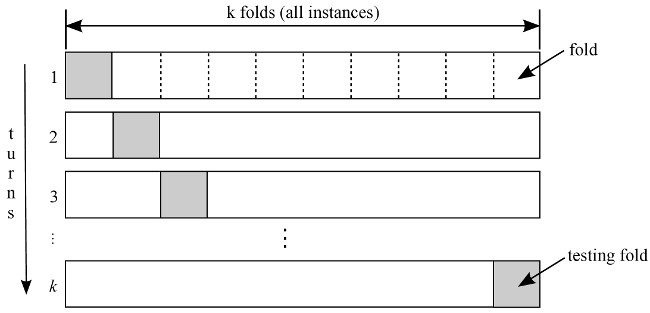
\includegraphics{k_folds}$$
	\caption{K-Folds Cross-Validation Example \cite{k_folds}}
	\label{fig:k_folds}
\end{figure}

\subsection{Training \& Testing Naive Bayes}
\label{training_and_testing_naive_bayes}

We utilize Scikit Learn's API for machine learning \cite{scikit} to create a \verb|pipeline|. In Scikit, \verb|pipelines| make managing machine learning algorithms easy by consolidating their parts into one object with configurable attributes.

\begin{minted}[linenos,fontsize=\scriptsize]{python}
sentiment_pipeline = Pipeline([
    ("vectorizer", TfidfVectorizer(tokenizer=tokenizer.tokenize,
                                   ngram_range=(1, 3),
                                   stop_words="english")),
    ("classifier", MultinomialNB())
])
\end{minted}

\noindent
Our \verb|pipeline| contains a vectorizer and a classifier. We change the default arguments for Scikit's TF-IDF vectorizer to use NLTK's tweet tokenizer, and specify that we want to calculate our TF-IDF vectors using unigrams, bigrams, and trigrams. Then, we set the vectorizer to use Scikit's default English language stop words. The Multinomial Naive Bayes Classifier we implement using Scikit includes \textbf{Laplace smoothing} ($\alpha=1$) by default. 

Scikit also has a convenient \verb|KFold| object which we utilize to perform cross-validation on our classifier. The goal of $k$-folds cross-validation is to train the classifier and acquire statistics on its performance while treating $k$ different parts of the ground truth dataset as \textbf{test sets}. Within a single iteration for 10 iterations, the \textbf{test set} will always be 10\% of the entire ground truth dataset, however the next iteration will use a different section. We ultimately average those statistics to understand the overall performance of the classifier. 

\begin{minted}[linenos,fontsize=\scriptsize]{python}
def confusion_matrices(training_data, num_folds=10):
    text_training_data = np.array([row[0] for row in training_data])
    class_training_data = np.array([row[1] for row in training_data])
    kf = KFold(n_splits=num_folds, random_state=42, shuffle=True)
    cnf_matrix_test = np.zeros((2, 2), dtype=int)
    for train_index, test_index in kf.split(text_training_data):
        text_train, text_test = (text_training_data[train_index], 
                                 text_training_data[test_index])
        class_train, class_test = (class_training_data[train_index], 
                                   class_training_data[test_index])

        sentiment_pipeline.fit(text_train, class_train)
        predictions_test = sentiment_pipeline.predict(text_test)
        cnf_matrix_test += confusion_matrix(class_test, predictions_test)
\end{minted}

\noindent
In each iteration of the 10 folds, the above program splits apart a training set and a \textbf{test set}. The classifier is trained on the \textbf{training set} using \verb|sentiment_pipeline.fit|, and the classifier's predictions for the \textbf{test set} in that fold are used to add toward a confusion matrix which will categorically visualize the performance of the classifier. We also calculate the \textbf{precision}, \textbf{recall}, and \textbf{$F_{1}$ score} for each fold's individual \textbf{test set}.

\section{Creating the Twitter Bot}
\label{creating_twitter_bot}

We use Tweepy to interact with the Twitter API. It provides a convenient object for streaming Twitter data in real time. The \verb|StreamListener| class can track tweets by searching for specific users, locations, and keywords. For our purposes, it has to be extended to track subtweets.

\begin{minted}[linenos,fontsize=\scriptsize]{python}
class StreamListener(tweepy.StreamListener):
    def on_status(self, status):
        id_str = status.id_str
        screen_name = status.user.screen_name
        created_at = status.created_at
        retweeted = status.retweeted
        in_reply_to = status.in_reply_to_status_id_str
        text = status.full_text
        
        # Genericize extra features and clean up the text
        text = (urls_pattern.sub("GENERIC_URL", 
                at_mentions_pattern.sub("GENERIC_MENTION", 
                names_pattern.sub("GENERIC_NAME",
                text)))
                .replace("\u2018", "'")
                .replace("\u2019", "'")
                .replace("\u201c", "\"")
                .replace("\u201d", "\"")
                .replace("&quot;", "\"")
                .replace("&amp;", "&")
                .replace("&gt;", ">")
                .replace("&lt;", "<"))
        
        tokens = tokenizer.tokenize(text)
        
        english_tokens = [english_dict.check(token) for token in tokens]
        percent_english_words = sum(english_tokens)/float(len(english_tokens))
        
        # Make sure the tweet contains some English
        is_english = False
        if percent_english_words >= 0.1:
            is_english = True
        
        # Calculate the probability using the pipeline
        subtweet_probability = sentiment_pipeline.predict_proba([text]).tolist()[0][1]
\end{minted}

\noindent
This part of the program is for live classification of subtweets and gathers information on tweet status objects as they are encountered. We extract data from the tweet object including the ID of that tweet and the text contained within it. We utilize the same techniques for cleaning and genericizing the tweet which we used in preparing our ground truth data for the classifier. The \verb|pipeline| has a \verb|predict_proba| method which takes as its input a list of strings and outputs an array of probabilities for each class. \verb|subtweet_probability|, then, uses that method to predict the probability that the tweet fits the ``subtweet" class according to the Naive Bayes classifier and the vectorizer we used in our \verb|pipeline|. We also check that the potential subtweet meets specific requirements before the Twitter bot will interact with it.

\begin{minted}[linenos,fontsize=\scriptsize]{python}
if all([subtweet_probability >= THRESHOLD,
        "RT" != text[:2], is_english, 
        not retweeted, not in_reply_to]):
\end{minted} 

\noindent
Included in this conditional statement is a comparison to determine if the probability that the tweet is a subtweet meets a specific threshold. We do not want to call out subtweets unless the probability is high enough. Following this check, we can interact with the tweet in several ways.

\begin{minted}[linenos,fontsize=\scriptsize]{python}
# Quote the tweet
api.update_status(("Is this a subtweet? {:.2%} \n" + 
                   "https://twitter.com/{}/status/{}").format(subtweet_probability, 
                                                              screen_name, 
                                                              id_str))
# Like the tweet
api.create_favorite(id_str)

# Reply to the tweet
api.update_status("@{} Is this a subtweet? {:.2%}".format(screen_name, 
                                                          subtweet_probability), 
                  id_str)
\end{minted}

\noindent
To quote the potential subtweet means that the tweet being referenced is embedded within our own tweet with a caption above it. Finally, we instantiate our custom \verb|StreamListener| class and use it to filter through tweets in real time.

\begin{minted}[linenos,fontsize=\scriptsize]{python}
stream_listener = StreamListener()
stream = tweepy.Stream(auth=api.auth, listener=stream_listener, tweet_mode="extended")

stream.filter(follow=user_ids, stall_warnings=True, languages=["en"], async=True)
print("Streaming has started.")
sleep(DURATION)
stream.disconnect()
\end{minted}

\noindent
The \verb|user_ids| list contains strings of Twitter user IDs. Every time a user whose ID is in the list sends a tweet, the program will classify that tweet and use the predicted probability that it is a subtweet to call it out on Twitter from the account linked to the application's API credentials. We filter the stream asynchronously in order to use the \verb|sleep| function from the \verb|time| Python library, so we can run the Twitter bot for a limited number of seconds.

\chapter{Results}
\label{results}

\section{Ground Truth Dataset}
\label{ground_truth_dataset}

No corpus already exists which provides examples of subtweets and non-subtweets. To produce such a corpus, the acquisition of the ground truth dataset relies on assumptions and generalizations of how Twitter users accuse others of subtweeting. For each subtweet and non-subtweet we acquired, we \textbf{did not} also acquire every single reply to that tweet, because doing so would violate the API's rate limits \cite{twitter_rate_limits}. Instead, we maintain that using Twitter's search API, a single reply to a tweet is enough to indicate that it \textbf{is} or \textbf{is not} a subtweet. By ignoring the associated metadata of tweet objects and their replies, we obtain the unicode text contained within subtweets and non-subtweets for our ground truth dataset.

\begin{center}
	\begin{tabular}{ | p{20em} | p{20em} | }
		\hline
		True Subtweets&True Non-Subtweets
		\\ 
		\hline
		I know who I want to take me home
		&
		He's followed the putrid smell of GENERIC\_MENTION which has led him to GENERIC\_MENTION's whereabouts. 

		Some odd neighbor boy was watching him as he approached the house. 
		Liam didn't hesitate to drink the young one dry. 

		``HONEY, I'M HOME!" 
		He calls, kicking in the door.
		\\ 
		\hline
		One bad chapter doesn't mean your story is over
		&
		YG so low? I guess the only group that sold physicals well is Bigbang GENERIC\_URL
		\\
		\hline
		What do you offer someone who doesn't like tea, coffee, or hot chocolate? YOU'RE A GUEST, YOU NEED A HOT DRINK, IT IS THE LAW.
		&
		is everything ok?? GENERIC\_URL
		\\
		\hline
		on the flip side, i agree that ``big" accounts have an obligation to do their due diligence to not sic their followers on others
		&
		The parade of falsehoods about CIA nominee Gina Haspel GENERIC\_URL
		\\
		\hline
		im bout to drop like 20lbs and then become a rapper.
		&
		Very first day of fortnite got 2 second place games and a third place gg not bad for a trash player :p
		\\
		\hline
		It's hilarious that your only ``godly" when it's convenient for you or when you want to put it on twitter. 
		&
		Rosie the Corpse Flower bloomed at Tucson Botanical Gardens: See pix allery here GENERIC\_URL \#Tucson GENERIC\_MENTION GENERIC\_URL
		\\
		\hline
		It really bothers me when people try to take advantage or assume I do shoots for free GENERIC\_URL
		&
		What is Uncle's GREATEST prediction?
		\\
		\hline
		I just don't get people lol
		&
		Didi Gregious is my new favorite player.
		\\
		\hline
		y'all kids today with your ``waifu this" and ``waifu that," back in my day our waifus had metal jaws and carried high-frequency blades
		&
		GENERIC\_MENTION we need to get you drawn as Dekamaster Doggy Krueger
		\\
		\hline
		I follow this gorgeous dog account on insta and his owner has such an annoying voice. SHUT UP AND LET ME ENJOY YOUR MAGNIFICENT DOG! I'M NOT HERE FOR YOU!
		&
		``Huge Caravan" Of Central Americans Is Headed For The U.S. Border In Hopes Of Asylum GENERIC\_URL
		\\
		\hline
	\end{tabular}
\end{center}

\noindent
When the vectorizer runs over these strings in order to tokenize them and extract features for use in the classifier, GENERIC\_URL, GENERIC\_MENTION, and GENERIC\_NAME stand in place of actual URLs, mentions of user names, and English first names in the original tweets. We use these generic tokens because we want the classifier to probabilistically acknowledge the presence of these features while specifically ignoring the content within them. 

\subsection{Characteristics of the Ground Truth Dataset}
\label{data_characteristics}

With tens of thousands of tweets contained within the ground truth dataset, understanding the characteristics of these tweets by example alone is insufficient. To improve our overall understanding of these characteristics, we gathered statistics on the distributions of tweet lengths, punctuating characters, stop words, and unique words in both the \textbf{true subtweets} and true \textbf{non-subtweets} parts of the dataset.

Twitter serves as a micro-blogging framework which limits the lengths of English text posts to 280 characters. Because Twitter is also a multimedia platform which supports embedding URLs, images, and videos, tweets do not necessarily contain this maximum number of characters. In contrast to the popularity of multimedia tweets, subtweets are characterized as exclusively text-based. Between both \textbf{true subtweets} and \textbf{true non-subtweets}, Figure \ref{fig:tweet_lengths} illustrates that the ground truth dataset contains more short tweets ($1\leq length \leq 125$) than long tweets ($125 < length \leq 280$). The subscripts $s$ and $n$ respectively indicate subtweets and non-subtweets.

\begin{figure}[H]
	$$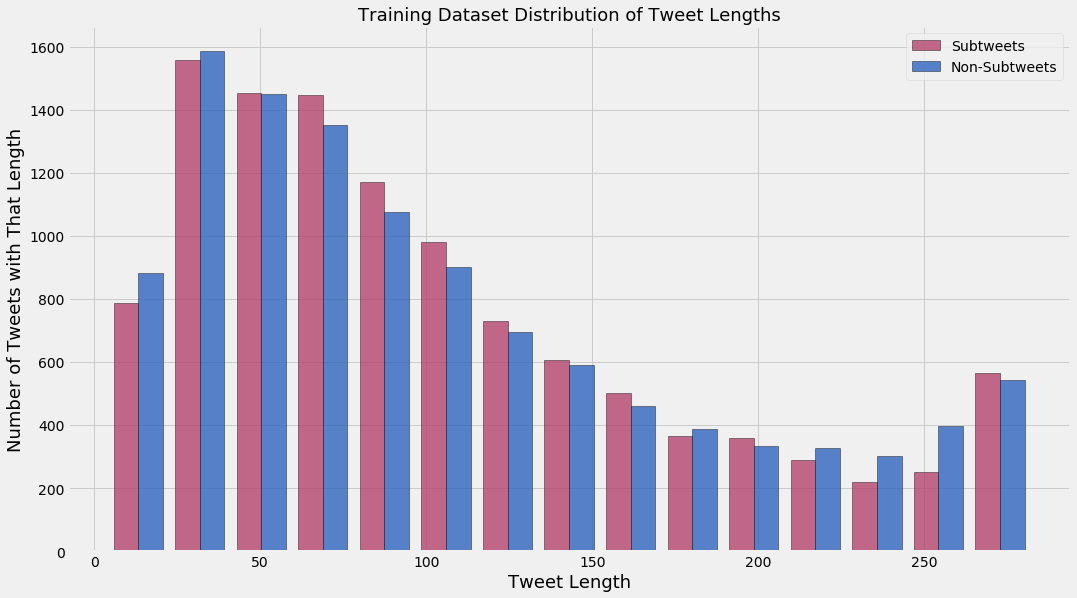
\includegraphics[width=\textwidth]{tweet_lengths_histogram.png}$$
	\caption{Histogram of Ground Truth Tweet Lengths 
	\\
	$(\bar{x}_{s}=103.71, s_{s}=71.99), (\bar{x}_{n}=105.63, s_{n}=74.95)$}
	\label{fig:tweet_lengths}
\end{figure}

Twitter does not enforce any grammar or syntax regulations in tweets, thus punctuating characters are often ignored altogether for use in the stream-of-consciousness style of writing. As shown in Figure \ref{fig:tweet_puncutation}, both \textbf{true subtweets} and \textbf{true non-subtweets} follow this trend in omitting punctuation, on average containing just under 2 punctuating characters (such as quotation marks, periods, commas, and apostrophes).

\begin{figure}[H]
	$$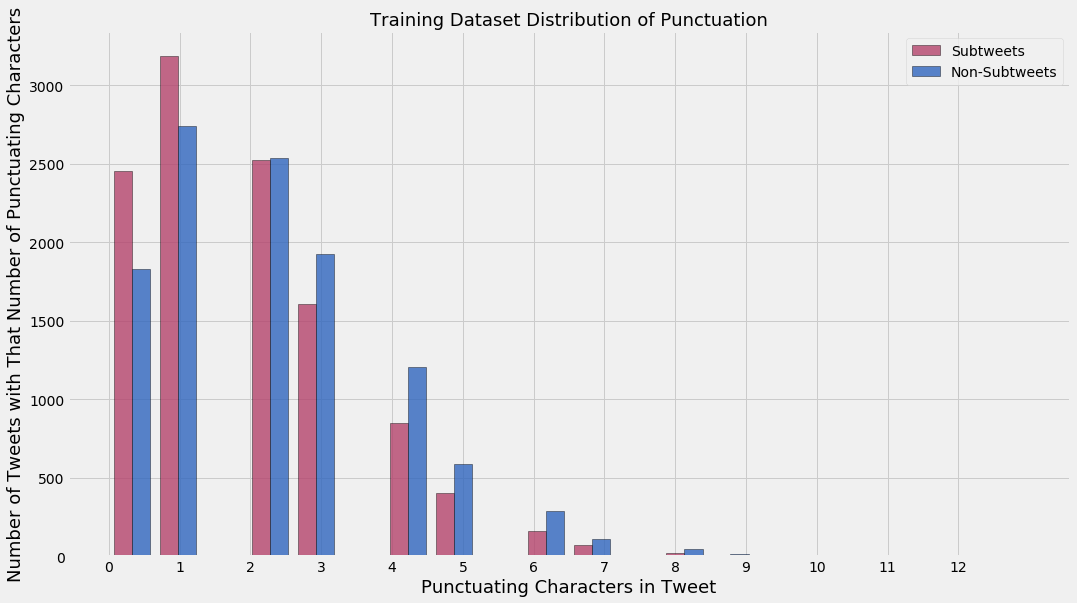
\includegraphics[width=\textwidth]{tweet_punctuations_histogram}$$
	\caption{Histogram of Ground Truth Tweet Punctuation
	\\
	$(\bar{x}_{s}=1.79, s_{s}=1.54), (\bar{x}_{n}=2.16, s_{n}=1.68)$}
	\label{fig:tweet_puncutation}
\end{figure}

English stop words are ignored by the vectorizer because they are too common to help the classifier distinguish between the appropriate features for the classes. Figure \ref{fig:tweet_stop_words} shows that our ground truth dataset contains tweets which are more likely to contain between 5 and 8 unique stop words than they are to contain fewer. In comparison, Figure \ref{fig:tweet_unique_words} illustrates the distribution of the number of \textbf{unique English words} per tweet in the ground truth dataset. As we expect of text-based posts under 280 characters in length, tweets containing fewer unique English words are more common.

\begin{figure}
	$$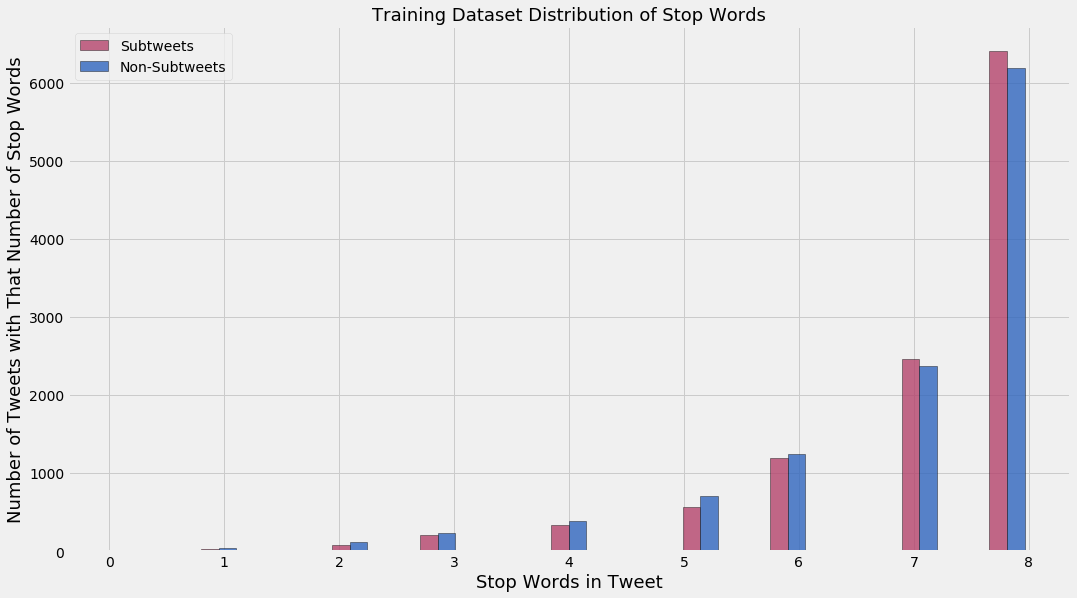
\includegraphics[width=\textwidth]{tweet_stop_words_histogram}$$
	\caption{Histogram of Ground Truth Unique English Stop Words
	\\
	$(\bar{x}_{s}=7.14, s_{s}=1.31), (\bar{x}_{n}=7.05, s_{n}=1.39)$
	}
	\label{fig:tweet_stop_words}
\end{figure}

\begin{figure}
	$$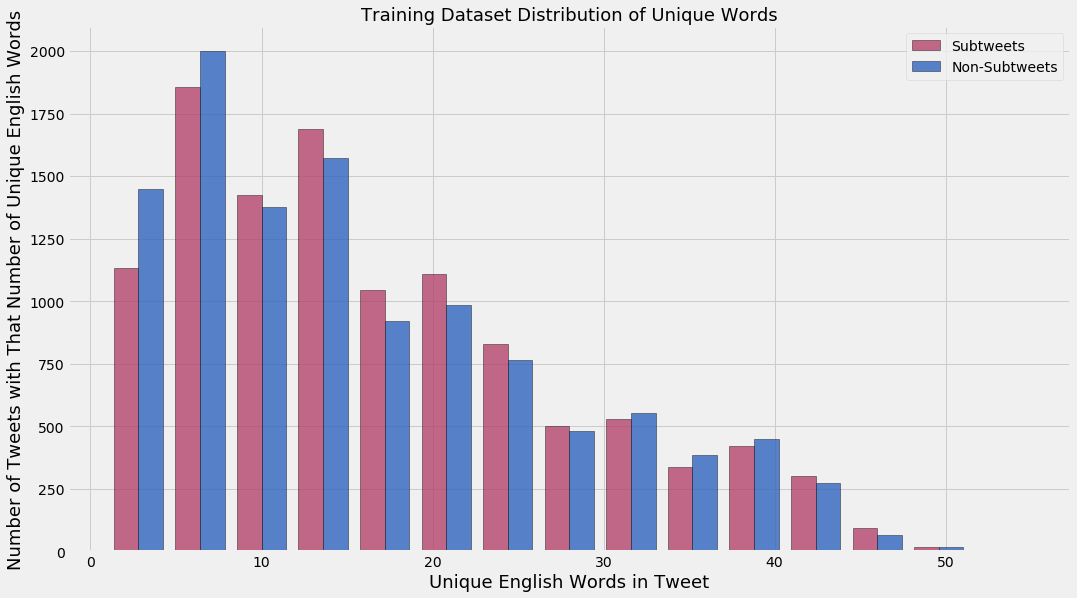
\includegraphics[width=\textwidth]{tweet_unique_words_histogram}$$
	\caption{Histogram of Ground Truth English Unique Words
	\\
	$(\bar{x}_{s}=16.80, s_{s}=10.95), (\bar{x}_{n}=16.25, s_{n}=11.15)$
	}
	\label{fig:tweet_unique_words}
\end{figure}

\section{Statistics}
\label{statistics}

\subsection{The Confusion Matrix}
\label{confusion_matrix}

We used $k$-folds cross-validation to test the performance of our Naive Bayes classifier on each \textbf{test set} fold of our ground truth dataset. Each individual \textbf{test set} was composed of only 10\% of the tweets in the entire dataset. By keeping track of the classifier's predictions on this \textbf{test set}, we accumulated a \textbf{confusion matrix} of \textbf{true positives}, \textbf{true negatives}, \textbf{false positives}, and \textbf{false negatives} for all 10 folds. Figure \ref{fig:confusion_matrix} illustrates these outcomes in terms of raw counts and normalized over the entire ground truth dataset.

\begin{figure}[H]
	$$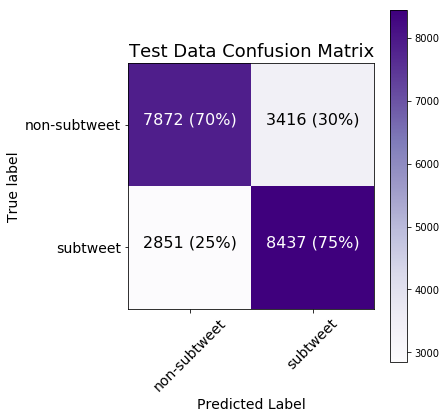
\includegraphics[width=20em]{confusion_matrix}$$
	\caption{Confusion Matrix on Test Data from Each Fold on the Ground Truth Dataset}
	\label{fig:confusion_matrix}
\end{figure}

We read the confusion matrix by matching rows with columns to see how well the classifier performs on \textbf{true subtweets} and \textbf{true non-subtweets} in making classifications to produce \textbf{predicted subtweets} and \textbf{predicted non-subtweets}. These results indicate that the Naive Bayes classifier performs 5\% better when classifying true positives than it does when classifying true negatives. In comparison, it is 5\% \textbf{worse} at classifying false positives than it is at classifying false negatives.

\subsection{Precision, Recall, \& F1}
\label{precision_etc}

The statistics gathered using $k$-folds cross-validation were averaged across all 10 folds, and measure the overall statistical performance of our classifier.

\begin{center}
	\begin{tabular}{ | p{7em} | p{4em} | p{4em} | p{4em} | }
		\hline
		&Precision&Recall&$F_{1}$ Score
		\\ 
		\hline
		Non-Subtweets&0.7357&0.6988&0.7166
		\\ 
		\hline
		Subtweets&0.7132&0.7490&0.7305
		\\
		\hline
	\end{tabular}
\end{center}

\noindent
The average $F_{1}$ scores for non-subtweets and subtweets are respectively 71.66\% and 73.05\%. Thus, our classifier performs similarly well above the 50\% \textbf{null accuracy} on both.

\section{Known Subtweeters}
\label{known_subtweeters_analysis}

In order to test how the classifier performed on tweets from known subtweeters, we acquired all publicly available tweets from 11 different accounts from which users had previously subtweeted. Figure \ref{fig:known_subtweeters} shows the distributions of tweets classified as subtweets under particular subtweet probability thresholds using the classifier on all the tweets from these accounts.

\begin{figure}[H]
	$$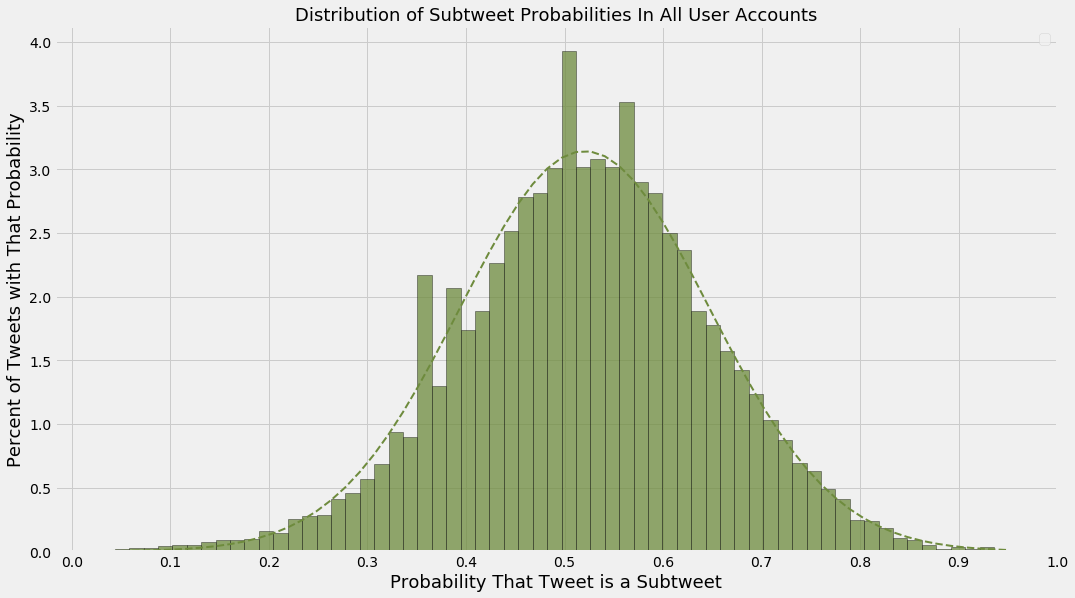
\includegraphics[width=\textwidth]{all_known_subtweeters_histogram}$$
	\caption{Distribution of Subtweet Probabilities for 11 Known Subtweeters 
	\\
	$(\bar{x}=0.520, s=0.127)$}
	\label{fig:known_subtweeters}
\end{figure}

Of these 11 accounts, the Naive Bayes classifier predicts that out of 26,928 tweets, 15,538 were subtweets (if the threshold for classifying a particular tweet as a subtweet was a probability of 50\%). In comparison, if we only accept classifications of at least 75\% and make that our threshold, then just 924 tweets (3.4\%) were predicted to be subtweets. Of these accounts, we selected the users who produced the minimum percentage of subtweets (27.6\%), the median percentage of subtweets (58.8\%), and the maximum percentage of subtweets (68.4\%) using the former (50\%) threshold. Figure \ref{fig:random_subtweeters} shows the distributions of tweets classified as subtweets under particular subtweet probability thresholds using the classifier for all the tweets from these three users' accounts.

\begin{figure}[H]
	$$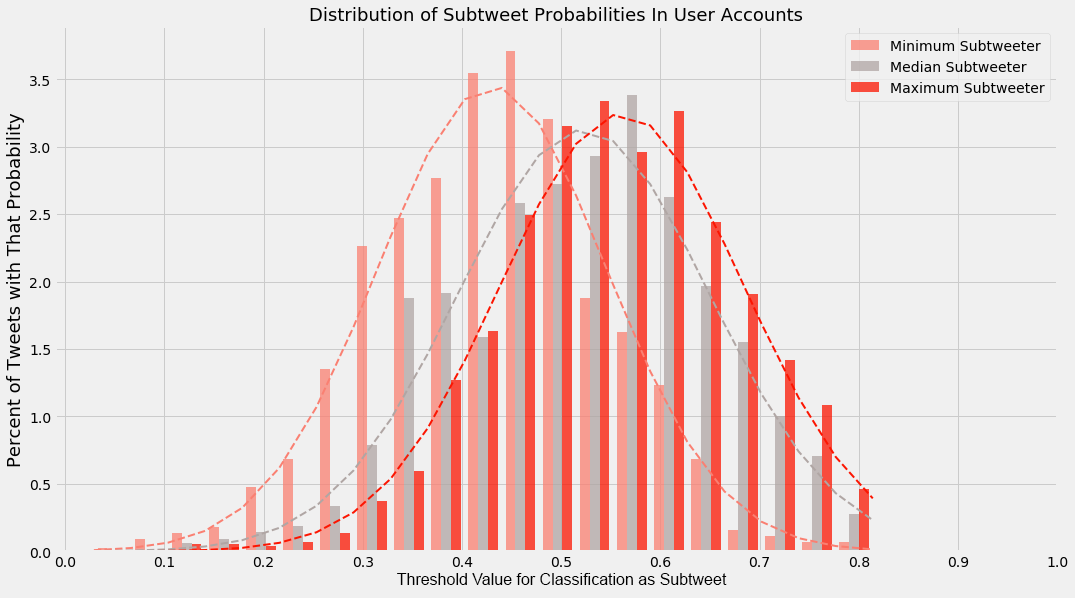
\includegraphics[width=\textwidth]{three_known_subtweeters_histogram}$$
	\caption{Distribution of Subtweet Probabilities for 3 Known Subtweeters 
	\\ 
	$(\bar{x}_{min}=0.430, s_{min}=0.116), (\bar{x}_{med}=0.523, s_{med}=0.128), (\bar{x}_{max}=0.561, s_{max}=0.123)$}
	\label{fig:random_subtweeters}
\end{figure}

\section{Most Informative Features}
\label{most_informative_features}

By iterating through the entire vocabulary of features on which the classifier was trained, and sorting those features by the probability that the feature belongs in the subtweet class, we are able to see which features are most informative for classifying tweets as \textbf{predicted subtweets}.

\begin{center}
\begin{tabular}{ | p{8em} | p{8.5em} | }
\hline
Token & $P(T|\omega=subtweet)$ \\ \hline
.       & -7.655 \\
,       & -8.022 \\
GENERIC\_URL& -8.049 \\
"       & -8.148 \\
people  & -8.427 \\
?       & -8.552 \\
like    & -8.673 \\
don't   & -8.683 \\
just    & -8.744 \\
i'm     & -8.833 \\
!       & -8.864 \\
it's    & -9.080 \\
. GENERIC\_URL   & -9.100 \\
:       & -9.110 \\
know    & -9.184 \\
...     & -9.204 \\
you're  & -9.210 \\
twitter & -9.284 \\
love    & -9.329 \\
*       & -9.404 \\
friends & -9.418 \\
\hline
\end{tabular}
\end{center}

\noindent
The only bigram in the top 20 most informative features is ``. GENERIC\_URL," which can only occur when a URL follows the end of a sentence. In comparison, the rest of these terms are unigrams of which 8 are exclusively punctuating characters (period, comma, quotation, question, exclamation mark, colon, ellipsis, and asterisk). The presence of these most informative features indicates the importance of punctuation in predicting subtweets. 

\section{The Twitter Bot}
\label{the_twitter_bot}

After training and testing our classifier, we utilized it in creation of a Twitter bot which interacts with \textbf{predicted subtweets} in real time. By limiting the minimum \textbf{predicted subtweet} probability threshold to 75\%, we prevent the Twitter bot from interacting with users too much. Figures \ref{fig:quotes_example} and \ref{fig:reply_example} show (censored) examples of these interactions.

\begin{figure}[H]
	$$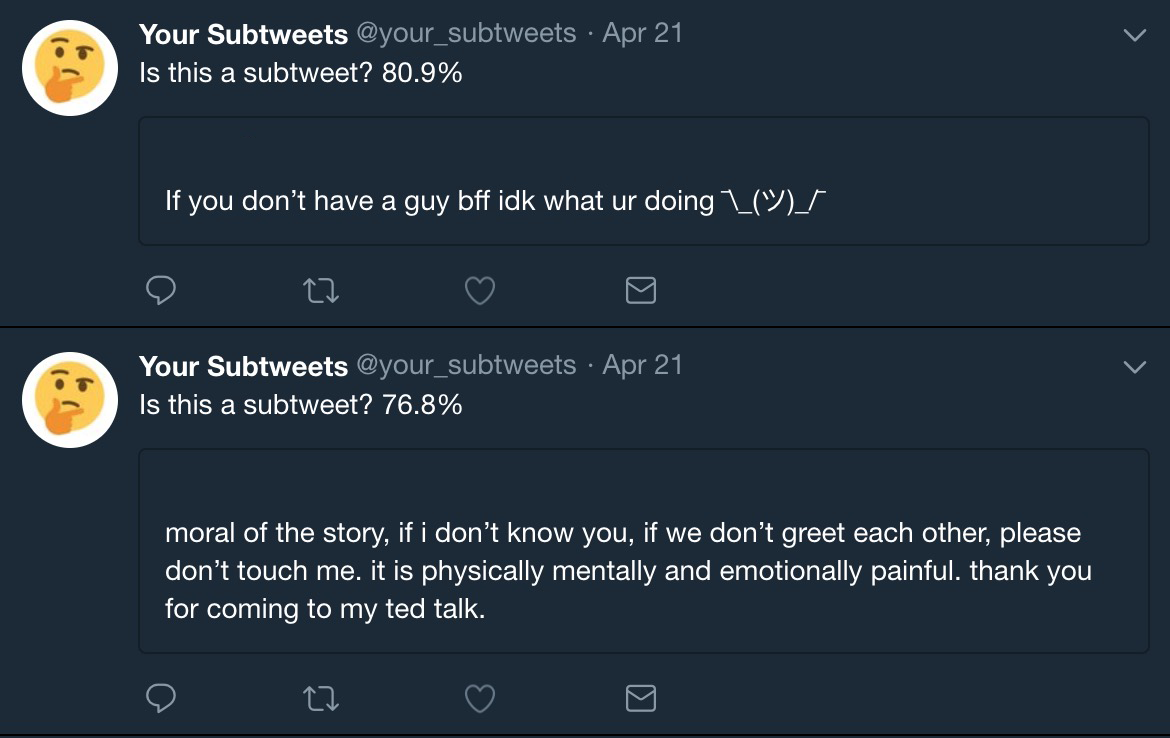
\includegraphics[width=30em]{quotes_example}$$
	\caption{Example of the Twitter Bot Quoting Users' Tweets}
	\label{fig:quotes_example}
\end{figure}

\begin{figure}[H]
	$$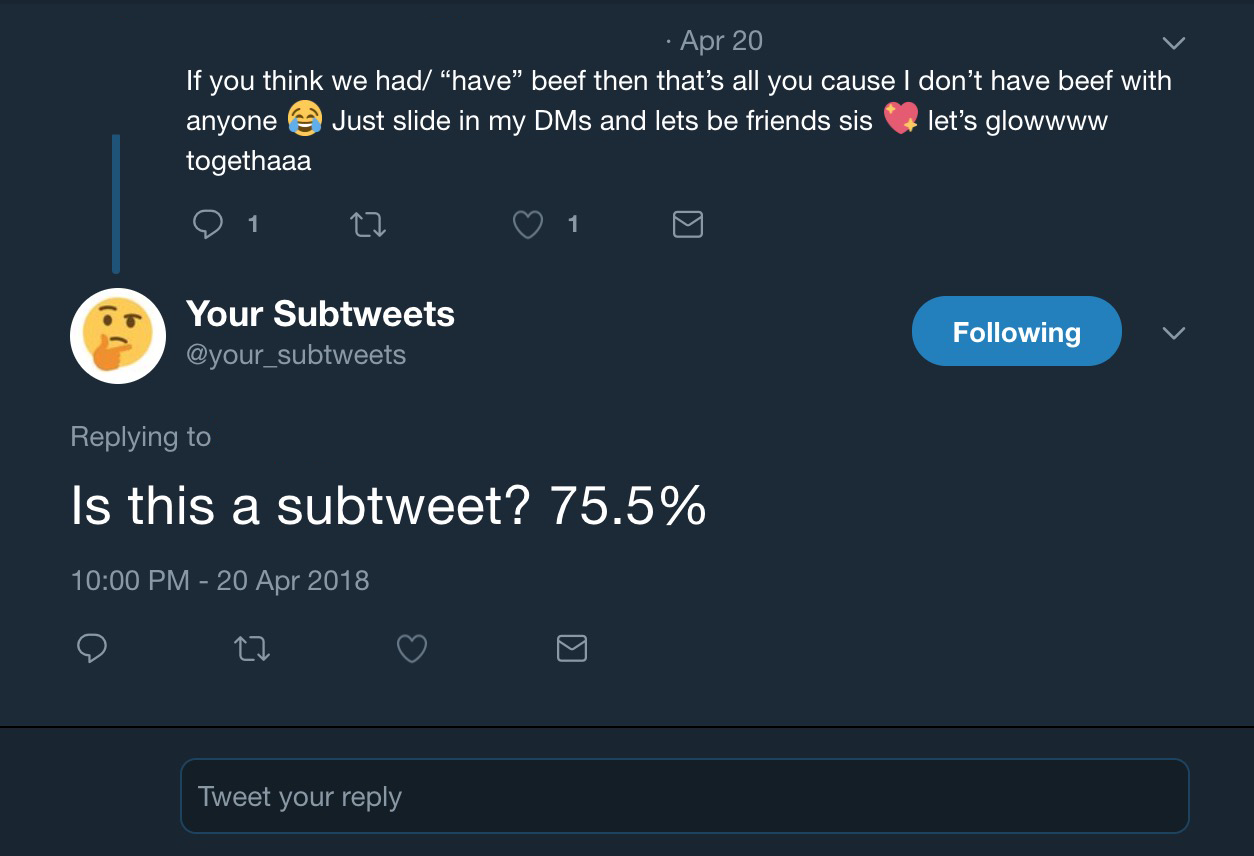
\includegraphics[width=30em]{reply_example}$$
	\caption{Example of the Twitter Bot Replying to a User's Tweet}
	\label{fig:reply_example}
\end{figure}

\section{Discussion}
\label{discussion}

Subtweets have garnered attention from news organizations \cite{the_atlantic}, social scientists \cite{subtweets_communications}, and governmental officials \cite{the_washington_post_trump}, but sentiment analysis of subtweets has been entirely unresearched. Utilizing the Twitter API, we acquired data for training and testing a Naive Bayes classifier, and developed a Twitter bot which actively calls-out subtweets in real time. We obtained 12,169 \textbf{true subtweets} and 21,411 \textbf{true non-subtweets} to be used in our ground truth dataset. After confirming they were English and removing duplicates, there were 11,288 \textbf{true subtweets} and 19,289 \textbf{true non-subtweets} remaining. In order to preserve a balance between the classes, we limited the number of \textbf{true non-subtweets} to be the same as the number of \textbf{true subtweets}. Thus, our final ground truth dataset contains 22,576 tweets. Our classifier identifies non-subtweets with an \textbf{$F_{1}$ score} of 71.66\% and subtweets with an \textbf{$F_{1}$ score} of 73.05\%, performing significantly better than the \textbf{null accuracy} of 50\%.

For the 2017 International Workshop on Semantic Evaluation (SemEval), numerous teams submitted approaches for task 4, subtask A: English Twitter polarity classification on a 3-point scale (\textbf{positive}, \textbf{neutral}, and \textbf{negative} sentiment) \cite{semeval_2017}. Although this particular classification is ternary instead of binary (such as in our case of classifying subtweets and non-subtweets), the outcomes of the competition on this particular subtask are still informative for us in comparing the performance of our method to others. The team which performed best on this subtask was \textbf{DataStories} with an average \textbf{$F_{1}$ score} of 67.7\% \cite{semeval_best}. Baziotis et al. utilized Long Short-Term Memory (LSTM) networks to achieve this score. In comparison to our average \textbf{$F_{1}$ score} of 72.4\%, we performed similarly well on a particularly less complicated problem than 3-point general sentiment classification.

Because we utilized our own novel method for data acquisition, we did not acquire a ground truth dataset which is as successful in representing the features of actual subtweets and non-subtweets as those which can be obtained using a service such as Amazon's Mechanical Turk which hand-labeled crowdsourced data. The Twitter API rate limitations prevented acquisition of tweets which were more than one week old at the time of downloading, and we only ever acquired one single reply to each subtweet and non-subtweet as the distinguishing characteristic of \textbf{true subtweets} and \textbf{true non-subtweets}. If a Twitter API search query exists which can find all the replies to a particular tweet, it will serve better than our method for finding only one.

\chapter{Conclusion}
\label{conclusion}

\section{Summary of Project Achievements}
\label{summary}

We treated a new colloquial form of online harassment---``subtweeting"---as a text classification problem and used the probabilistic Naive Bayes classification algorithm to identify it. We judged the performance of the algorithm and went beyond identification to engage with subtweets, promoting publicity for content which is deliberately written to be unseen by the targeted party. We utilized Twitter's API to demonstrate a potential use for sentiment analysis on this kind of text.
\linebreak
\linebreak
\noindent
All data acquired and all programs developed for this project have been made publicly available on GitHub at \url{https://github.com/segalgouldn/Senior-Project-Subtweets}.

\section{Future Work \& Considerations}
\label{future_work_and_considerations}

Our implementation of Naive Bayes exclusively made classifications using features from the unicode text contained within tweets, but other features related to the metadata contained within tweet objects and their replies will probably prove fruitful in producing a better subtweets classifier. We did not test other classification algorithms in favor of pursuing Naive Bayes singularly, but there exists no reason to \textbf{not} utilize others. Using topic modeling via methods such as non-negative matrix factorization and latent dirichlet allocation, we can analyze the topics about which most users are tweeting, and potentially group these users into subtweet-topic networked communities through clustering algorithms such as $k$-means.

Finally, we treated this project as a binary classification problem between subtweets and non-subtweets, but it can be expanded. What would we find if we trained a classifier to distinguish ironic tweets, sarcastic tweets, mocking tweets, and subtweets? What are the features of the figurative language used in each of these examples? These questions motivate further research.

\begin{bibliog}

\bib{antilocution}{article}{
	title={The nature of prejudice},
	author={Allport, Gordon W},
	date={1954}
}

\bib{semeval_best}{article}{
  title={Datastories at SemEval-2017 task 4: Deep LSTM with attention for message-level and topic-based sentiment analysis},
  author={Baziotis, Christos},
  author={Pelekis, Nikos},
  author={Doulkeridis, Christos},
  journal={Proceedings of the 11th International Workshop on Semantic Evaluation (SemEval-2017)},
  pages={747\ndash754},
  date={2017}
}

\bib{nltk}{article}{
	title={NLTK: the natural language toolkit},
	author={Bird, Steven},
	author={Loper, Edward},
	journal={Proceedings of the ACL 2004 on Interactive poster and demonstration sessions},
	pages={31},
	date={2004}
}

\bib{k_folds}{article}{
	author={Borovicka, Tomas},
	author={Jirina Jr, Marcel},
	author={Kordik, Pavel},
	author={Jirina, Marcel},
	title={Selecting representative data sets},
	date={2012}
}

\bib{sentiment_analysis_terrorism}{article}{
	author={Burnap, Pete},
	author={Williams, Matthew~L},
	author={Sloan, Luke},
	author={Rana, Omer},
	author={Housley, William},
	author={Edwards, Adam},
	author={Knight, Vincent},
	author={Procter, Rob},
	author={Voss, Alex},
	title={Tweeting the terror: modelling the social media reaction to the woolwich terrorist attack},
	date={2014},
	journal={Social Network Analysis and Mining},
	volume={4},
	number={1},
	pages={206},
}

\bib{the_washington_post}{article}{
	author={Dewey, Caitlin},
	title={Study confirms what you always knew: People who subtweet are terrible},
	date={2016},
	eprint={https://goo.gl/SeV3mx},
}

\bib{first_tweet}{article}{
	author={Dorsey, Jack},
	title={inviting coworkers},
	date={2006},
	eprint={https://twitter.com/jack/status/29},
}

\bib{subtweets_communications}{article}{
	author={Edwards, Autumn},
	author={Harris, Christina~J},
	title={To tweet or ‘subtweet’?: Impacts of social networking post directness and valence on interpersonal impressions},
	date={2016},
	journal={Computers in Human Behavior},
	volume={63},
	pages={304\ndash 310},
}

\bib{semeval_2015}{article}{
	title={Semeval-2015 task 11: Sentiment analysis of figurative language in twitter},
	author={Ghosh, Aniruddha},
	author={Li, Guofu}, 
	author={Veale, Tony},
	author={Rosso, Paolo}, 
	author={Shutova, Ekaterina}, author={Barnden, John}, 
	author={Reyes, Antonio},
	journal={Proceedings of the 9th International Workshop on Semantic Evaluation (SemEval 2015)},
	pages={470\ndash478},
	year={2015}
}

\bib{go_dataset}{article}{
	title = {Twitter Sentiment Classification using Distant Supervision},
	author = {Go, Alec},
	author = {Bhayani, Richa},
	author = {Huang, Lei},
	journal = {CS224N Project Report, Stanford},
	pages = {12},
	date = {2009}
}

\bib{slate}{article}{
	author={Hassler, Chelsea},
	title={Subtweeting looks terrible on you. (you know who you are.)},
	date={2016},
	eprint={https://goo.gl/NCz27z},
}

\bib{pyenchant}{article}{
	title={PyEnchant: a spellchecking library for Python},
	author={Kelly, Ryan},
	date={2016}
}

\bib{the_atlantic}{article}{
	author={Madrigal, Alexis~C.},
	title={Behind the machine's back: How social media users avoid getting turned into big data},
	date={2014},
	eprint={https://goo.gl/h36jxx},
}

\bib{sentiment_survey}{article}{
	title={Sentiment analysis algorithms and applications: A survey},
	author={Medhat, Walaa},
	author={Hassan, Ahmed},
	author={Korashy, Hoda},
	journal={Ain Shams Engineering Journal},
	volume={5},
	number={4},
	pages={1093\ndash1113},
	date={2014},
}

\bib{sentiment_analysis_markets}{article}{
	author={Nassirtoussi, Arman~Khadjeh},
	author={Aghabozorgi, Saeed},
	author={Wah, Teh~Ying},
	author={Ngo, David Chek~Ling},
	title={Text mining for market prediction: A systematic review},
	date={2014},
	journal={Expert Systems with Applications},
	volume={41},
	number={16},
	pages={7653\ndash 7670},
}

\bib{the_washington_post_trump}{article}{
	author={Ohlheiser, Abby},
	title={A running list of all the possible subtweets of President Trump from government Twitter accounts},
	date={2017},
	eprint={https://goo.gl/hFh81R},
}

\bib{scikit}{article}{
	title={Scikit-learn: Machine learning in Python},
	author={Pedregosa, Fabian},
	author={Varoquaux, Ga{\"e}l},
	author={Gramfort, Alexandre},
	author={Michel, Vincent}, 
	author={Thirion, Bertrand},
	author={Grisel, Olivier},
	author={Blondel, Mathieu}, 
	author={Prettenhofer, Peter},
	author={Weiss, Ron},
	author={Dubourg, Vincent},
	journal={Journal of machine learning research},
	volume={12},
	number={Oct},
	pages={2825--2830},
	date={2011}
}

\bib{first_subtweet}{article}{
	author={Rae, Chelsea},
	title={I hate when i see people...},
	date={2009},
	eprint={https://twitter.com/Chelsea_x_Rae/status/6261479092},
}

\bib{tweepy_python}{article}{
	title={tweepy Documentation},
	author={Roesslein, Joshua},
	eprint={http://docs.tweepy.org/en/v3.5.0/},
	volume={5},
	date={2009}
}

\bib{semeval_2017}{article}{
	title={SemEval-2017 task 4: Sentiment analysis in Twitter},
	author={Rosenthal, Sara},
	author={Farra, Noura}, 
	author={Nakov, Preslav},
  	journal={Proceedings of the 11th International Workshop on Semantic Evaluation (SemEval-2017)},
  	pages={502\ndash518},
  	date={2017}
}

\bib{twitter_api_start}{article}{
	author={Stone, Biz},
	title={Introducing the Twitter API},
	date={2006},
	eprint={https://blog.twitter.com/official/en_us/a/2006/introducing-the-twitter-api.html},
}

\bib{twitter_api_docs}{article}{
	author={Twitter},
	title={Twitter API Docs},
	date={2018},
	eprint={https://developer.twitter.com/en/docs},
}

\bib{twitter_tos}{article}{
	author={Twitter},
	title={Twitter Terms of Service},
	date={2016},
	eprint={https://twitter.com/en/tos}
}

\bib{tweepy_status_object}{article}{
	author={Twitter},
	title={Tweet objects},
	date={2018},
	eprint={https://developer.twitter.com/en/docs/tweets/data-dictionary/overview/tweet-object},
}

\bib{twitter_stats}{article}{
	author={Twitter},
	title={Twitter turns six},
	date={2012},
	eprint={https://blog.twitter.com/official/en_us/a/2012/twitter-turns-six.html},
}

\bib{twitter_rate_limits}{article}{
	author={Twitter},
	title={Rate Limiting},
	date={2018},
	eprint={https://developer.twitter.com/en/docs/basics/rate-limiting},
}

\bib{urban_dictionary}{article}{
	author={Urban Dictionary},
	title={Subtweet},
	date={2010},
	eprint={https://www.urbandictionary.com/define.php?term=subtweet},
}

\bib{semeval_2018}{article}{
	author={Van Hee, Cynthia}, 
	author={Lefever, Els}, 
	author={Host, Véronique},
	title={Semeval-2018 Task 3: Irony detection in English Tweets},
	date={2018},
	journal={Proceedings of the 12th International Workshop on Semantic Evaluation (SemEval-2018)}
}

\bib{naive_bayes_optimality}{article}{
	title={The optimality of naive Bayes},
	author={Zhang, Harry},
	journal={AA},
	volume={1},
	number={2},
	pages={3},
	date={2004}
}

\end{bibliog}

\end{document}

% end of file bardproj_template.tex
